
\begin{frame}
\frametitle{Introduction}
\framesubtitle{FGT Demo}


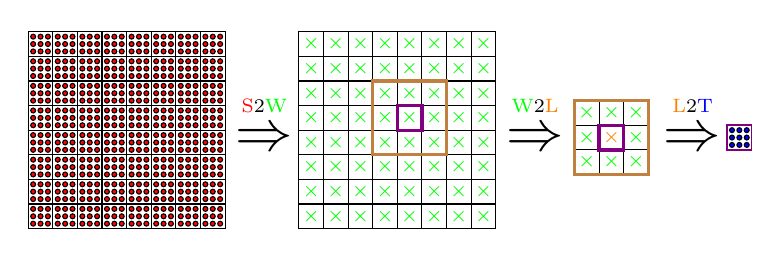
\begin{tikzpicture}[scale=1.25]

\draw (0,0) rectangle (2,2);

\foreach \ypos in {0.25, 0.5, ..., 1.75} {
 \draw (0, \ypos) -- (2, \ypos);
}

\foreach \xpos in {0.25, 0.5, ..., 1.75} {
 \draw (\xpos, 0) -- (\xpos, 2);
}

\foreach \xpos in {0, 0.25, ..., 1.75} {
 \foreach \ypos in {0, 0.25, ..., 1.75} {
  \foreach \apos in {0.05, 0.125, 0.2} {
  \foreach \bpos in {0.05, 0.125, 0.2} {
   \draw[fill = red] (\xpos, \ypos) ++(\apos, \bpos) circle (0.025); 
   }
  }
 }
}

\draw (2.4, 0.9) node {\huge{$\Rightarrow$}};
\draw (2.4, 1.25) node {\scriptsize{{\color{red}{S}}2{\color{green}{W}}}};

\draw (2.75,0) rectangle (4.75,2);

\foreach \ypos in {0.25, 0.5, ..., 1.75} {
 \draw (2.75, \ypos) -- (4.75, \ypos);
}

\foreach \xpos in {3.0, 3.25, ..., 4.5} {
 \draw (\xpos, 0) -- (\xpos, 2);
}

\foreach \xpos in {2.75, 3.0, ..., 4.5} {
 \foreach \ypos in {0, 0.25, ..., 1.75} {
   \draw[green] (\xpos, \ypos) ++(0.125, 0.125) node {\scriptsize{$\times$}};   
 }
}

\draw[violet, very thick] (3.75, 1) rectangle +(0.25, 0.25);
\draw[brown, very thick] (3.5, 0.75) rectangle +(0.75, 0.75);

\draw (5.15, 0.9) node {\huge{$\Rightarrow$}};
\draw (5.15, 1.25) node {\scriptsize{{\color{green}{W}}2{\color{orange}{L}}}};

\draw (5.55, 0.55) ++(0, 0.25) -- +(0.75, 0);
\draw (5.55, 0.55) ++(0, 0.5) -- +(0.75, 0);
\draw (5.55, 0.55) ++(0.25, 0) -- +(0, 0.75);
\draw (5.55, 0.55) ++(0.5, 0) -- +(0, 0.75);

\draw[violet, very thick] (5.8, 0.8) rectangle +(0.25, 0.25);
\draw[brown, very thick] (5.55, 0.55) rectangle +(0.75, 0.75);

\draw[green] (5.55, 0.55) ++(0.125, 0.125) node {\scriptsize{$\times$}};   
\draw[green] (5.55, 0.55) ++(0.375, 0.125) node {\scriptsize{$\times$}};   
\draw[green] (5.55, 0.55) ++(0.625, 0.125) node {\scriptsize{$\times$}};   

\draw[green] (5.55, 0.55) ++(0.125, 0.375) node {\scriptsize{$\times$}};   
\draw[orange] (5.55, 0.55) ++(0.375, 0.375) node {\scriptsize{$\times$}};   
\draw[green] (5.55, 0.55) ++(0.625, 0.375) node {\scriptsize{$\times$}};   

\draw[green] (5.55, 0.55) ++(0.125, 0.625) node {\scriptsize{$\times$}};   
\draw[green] (5.55, 0.55) ++(0.375, 0.625) node {\scriptsize{$\times$}};   
\draw[green] (5.55, 0.55) ++(0.625, 0.625) node {\scriptsize{$\times$}};   

\draw (6.75, 0.9) node {\huge{$\Rightarrow$}};
\draw (6.75, 1.25) node {\scriptsize{{\color{orange}{L}}2{\color{blue}{T}}}};

\draw[violet, line width = 0.2mm] (7.1, 0.8) rectangle +(0.25, 0.25);

\foreach \apos in {0.05, 0.125, 0.2} {
 \foreach \bpos in {0.05, 0.125, 0.2} {
  \draw[fill = blue] (7.1, 0.8) ++(\apos, \bpos) circle (0.025); 
  }
}


\end{tikzpicture}

\vspace{0.4cm}

\begin{description}
\item[{\textbf{{\color{red}{S}}{\color{black}{2}}{\color{green}{W}}}} \hspace{1cm}] 
$ {\color{green}{w_k}} = \displaystyle{\sum_{{\color{red}{y}} \in {\color{green}{B}}}} f({\color{red}{y}})  
  e^{i\lambda k \cdot ({\color{green}{c^B}} - {\color{red}{y}})} \quad \forall\quad |k| \leq p $            
\newline
\item[{\textbf{{\color{green}{W}}{\color{black}{2}}{\color{orange}{L}}}} \hspace{1cm}] 
$ {\color{orange}{v_k}} += {\color{green}{w_k}} e^{i\lambda k \cdot ({\color{orange}{c^D}} - {\color{green}{c^B}})} $            
\newline
\item[{\textbf{{\color{orange}{L}}{\color{black}{2}}{\color{blue}{T}}}} \hspace{1cm}] 
$ F({\color{blue}{x}}) = \displaystyle{\sum_{|k| \leq p}} \hat{G}(k) {\color{orange}{v_k}}
  e^{i\lambda k \cdot ({\color{blue}{x}} - {\color{orange}{c^D}})} $
\end{description} 


\end{frame}

